Arhitektura i dizajn sustava}
		
		{Arhitekturu možemo podijeliti na 3 podsustava:}

		\begin{packed_item}
			\item {Web poslužitelj}
			\item {Web aplikacija}
			\item {Baza podataka}\vspace{0.1cm}
		\end{packed_item}
	
		{\underbar{Web preglednik} (\textit{Internetski preglednik, Web browser, Internet browser})  je program koji korisniku omogućuje pregled web-stranica i multimedijalnih sadržaja vezanih uz njih. Svaki internetski preglednik je \underbar{interpreter} (program koji u realnom vremenu izvršava izvorni kod napisan u nekom programskom jeziku, umjesto da ga, prije izvršavanja cijelog prevede u strojni jezik, što inače radi jezični prevoditelj). Dakle, stranica je pisana u kodu koji preglednik interpretira u čitljiv sadržaj. Korisnici putem web preglednika šalju zahtjeve Web poslužitelju.}\vspace{0.3cm}

		{\underbar{Web poslužitelj} je temelj svake Web aplikacije jer on služi za komunikaciju klijenta s aplikacijom. Takva vrsta komunikacije odvija se uz pomoć HTTP (\textit{Hyper Text Transfer Protocol}) protokola koji predstavlja glavnu i najčešću metodu prijenosa informacija na Webu. Osnovna namjena ovog protokola je omogućavanje objavljivanja i prezentacije HTML dokumenata, tj. Web stranica. Web poslužitelj nam dakle služi za prosljeđivanje zahtjeva Web aplikaciji te je zadužen za njezino pokretanje.}\vspace{0.3cm}

		{Od ostalih protokola koji služe za komunikaciju i prijenos informacija i podataka između klijenta i poslužitelja treba napomenuti: IP (\textit{Internet Protocol}) koji služi za prijenos podataka u blokovima (paketi, datagrami), komunikacijski protokol ARP (\textit{Address Resolution Protocol}) te ICMP (\textit{Internet Control Message Protocol}) koji je ugrađen u svaki IP modul kako bi omogućio računalima slanje kontrolnih poruka o greškama. ICMP prijavljuje greške, ali nije zadužen za njihovo ispravljanje.}\vspace{0.3cm}

		{Klijent koristi Web aplikaciju za obradu traženih zahtjeva. Aplikacija vrši obradu zahtjeva te, u slučaju pozitivnog ishoda obrade, pristupa bazi podataka. Nakon toga preko Web poslužitelja vraća korisniku odgovor koji mu je razumljiv i vidljiv u Web pregledniku.}\vspace{0.3cm}

		{Programski i korisnički jezici koje smo koristili su: HTML, CSS i JavaScript za Frontend te Java za Backend. Radni okviri koje smo odabrali su React (Frontend) i Spring Boot (Backend). Od razvojnih okruženja koristili smo IntelliJ u okviru izrade Backenda te Visual Studio Code za izradu Frontenda.}\vspace{0.3cm}

		{U okviru Backenda korišten je REST (\textit{Representational State Transfer}) API (\textit{Application programming Interface}). \underbar{REST} je softverska arhitektura koja nameće uvjete o tome kako API treba raditi, a \underbar{API} definira pravila koja morate slijediti za komunikaciju s drugim softverskim sustavima.}\vspace{0.3cm}

		{\underbar{REST API} je sučelje koje dva računalna sustava koriste za sigurnu razmjenu informacija putem interneta. Većina Web aplikacija mora komunicirati s drugim internim aplikacijama i aplikacijama trećih strana kako bi izvršile razne zadatke, a REST API podržava ovu razmjenu informacija jer slijedi sigurne, pouzdane i učinkovite softverske komunikacijske standarde.}\pagebreak
		


				
		\section{Baza podataka}
			
			\textbf{\textit{dio 1. revizije}}\\
			
		\textit{Podaci u našoj aplikaciji će se spremati u relacijsku bazu podataka koristeći Postgres kao DBMS. Baza će se sastojati od sljedećih entiteta:}
		\begin{itemize}
			\item Korisnik
			\item Tvrtka
			\item Projekt
			\item ProjectFRTeamMembers
			\item Mjesto
			\item Zaposlenik
			\item Suradnja
		\end{itemize}
			\subsection{Opis tablica}

				\begin{longtblr}[
					label=none,
					entry=none
					]{
						width = \textwidth,
						colspec={|X[14,l]|X[8, l]|X[20, l]|}, 
						rowhead = 1,
					} %definicija širine tablice, širine stupaca, poravnanje i broja redaka naslova tablice
						\hline \multicolumn{3}{|c|}{\textbf{Korisnik}}	 \\ \hline[3pt]
						\SetCell{LightGreen}IDKorisnik & INT & ID kosisnika  	\\ \hline
						Ime	& VARCHAR & Ime korisnika \\ \hline 
						Prezime & VARCHAR & Prezime korisnika \\ \hline 
						Nadimak & VARCHAR	& Nadimak korisnika \\ \hline 
		        				LoginEmail & VARCHAR	& Email adresa pomoću kojeg se user logira \\ \hline 
		        				NotificationEmail & VARCHAR	& Email adresa na koju korisnik prima obavijesti \\ \hline 
						MaxRazinaOvlasti & VARCHAR & Maksimalna razina ovlasti na projektima \\ \hline
				\end{longtblr}

				\begin{longtblr}[
					label=none,
					entry=none
					]{
						width = \textwidth,
						colspec={|X[14,l]|X[8, l]|X[20, l]|}, 
						rowhead = 1,
					} %definicija širine tablice, širine stupaca, poravnanje i broja redaka naslova tablice
					\hline \multicolumn{3}{|c|}{\textbf{Mjesto}}	 \\ \hline[3pt]
					\SetCell{LightGreen} PostanskiBrojGrad & VARCHAR & Poštanski broj grada \\ \hline
					NazivGrad & VARCHAR & Naziv grada \\ \hline
				\end{longtblr}

				\begin{longtblr}[
					label=none,
					entry=none
					]{
						width = \textwidth,
						colspec={|X[14,l]|X[8, l]|X[20, l]|}, 
						rowhead = 1,
					} %definicija širine tablice, širine stupaca, poravnanje i broja redaka naslova tablice
						\hline \multicolumn{3}{|c|}{\textbf{Tvrtka}}	 \\ \hline[3pt]
						\SetCell{LightGreen} IdTvrtka & INT	&  Id tvrtke	\\ \hline
						Naziv & VARCHAR & Naziv tvrtke \\ \hline 
						Podrucje & VARCHAR &  Područje kojim se tvrtka bavi \\ \hline 
						ABCKategorija & CHAR & Kategorija tvrtke (A B ili C) \\ \hline 
				                     MjesecPlaniranjaBudzeta & INT & Mjesec u kojem tvrtka planira budžet \\ \hline
				                     Drzava & VARCHAR & Država u kojoj tvrtka posluje \\ \hline
				                     \SetCell{LightBlue} PBr & VARCHAR & Poštanski broj mjesta tvrtke \\ \hline
						Adresa & VARCHAR & Adresa tvrtke \\ \hline
				                 	WebStranica & VARCHAR & Adresa web stranice tvrtke \\ \hline
					           Kontaktirati & BOOLEAN & Treba li ubuduće tu tvrtku treba kontaktirati \\ \hline
				\end{longtblr}

				\begin{longtblr}[
					label=none,
					entry=none
					]{
						width = \textwidth,
						colspec={|X[14,l]|X[8, l]|X[20, l]|}, 
						rowhead = 1,
					} %definicija širine tablice, širine stupaca, poravnanje i broja redaka naslova tablice
					\hline \multicolumn{3}{|c|}{\textbf{Zaposlenik}}	 \\ \hline[3pt]
						\SetCell{LightGreen} IDZaposlenik & INT	& Id zaposlenika \\ \hline
						\SetCell{LightBlue} IDTvrtke & INT & Id tvrtke za koju zaposlenik radi\\ \hline 
						Ime & VARCHAR & Ime zaposlenika \\ \hline 
						Prezime & VARCHAR	& Prezime zaposlenika \\ \hline 
				                    Email & VARCHAR	& Email adresa zaposlenika \\ \hline 
				                    BrojTelefona & VARCHAR	& Broj telefona zaposlenika \\ \hline 
				                    Uloga & VARCHAR	& Pozicija zaposlenika u tvrtci (npr. PR) \\ \hline 
				                    Opis & VARCHAR	& Opis zaposlenika (npr. glavni kontakt) \\ \hline 
				\end{longtblr}

				\begin{longtblr}[
					label=none,
					entry=none
					]{
						width = \textwidth,
						colspec={|X[14,l]|X[8, l]|X[20, l]|}, 
						rowhead = 1,
					} %definicija širine tablice, širine stupaca, poravnanje i broja redaka naslova tablice
					\hline \multicolumn{3}{|c|}{\textbf{Projekt}}	 \\ \hline[3pt]
					\SetCell{LightGreen}IDProjekt & INT	& Id projekta \\ \hline
					Naziv & VARCHAR & Naziv projekta \\ \hline 
					KategorijaProjekta & INT & Kategorija u koju spada projekt \\ \hline 
					TipProjekta & INT & Eksterni ili interni projekt \\ \hline 
					DatumPočetka & TIMESTAMP & Datum početka projekta \\ \hline 
				                DatumZavršetka & TIMESTAMP & Datum završetka projekta \\ \hline 
				                \SetCell{LightBlue} FRResponsibleUserId & INT & Id korisnika odgovornog za odnose s tvrtkama projekta \\ \hline
				                FRCilj & INT & Količina novca koja se želi prikupiti za projekt \\ \hline
				                FirstPing & TIMESTAMP & Datum prvog "ping"-a \\ \hline
				                SecondPing & TIMESTAMP & Datum drugog "ping"-a \\ \hline
				\end{longtblr}

				\begin{longtblr}[
					label=none,
					entry=none
					]{
						width = \textwidth,
						colspec={|X[14,l]|X[8, l]|X[20, l]|}, 
						rowhead = 1,
					} %definicija širine tablice, širine stupaca, poravnanje i broja redaka naslova tablice
					\hline \multicolumn{3}{|c|}{\textbf{ProjectFRTeamMembers}}	 \\ \hline[3pt]
					\SetCell{LightGreen}IDKorisnik & INT & Id korisnika koji je FR team member projekta \\ \hline
					\SetCell{LightGreen}IDProjekt & INT & Id projekta \\ \hline
				\end{longtblr}

				\begin{longtblr}[
					label=none,
					entry=none
					]{
						width = \textwidth,
						colspec={|X[14,l]|X[8, l]|X[20, l]|}, 
						rowhead = 1,
					} %definicija širine tablice, širine stupaca, poravnanje i broja redaka naslova tablice
					\hline \multicolumn{3}{|c|}{\textbf{Suradnja}}	 \\ \hline[3pt]
					\SetCell{LightGreen}IDProjekt & INT	& Id projekta \\ \hline
			                \SetCell{LightGreen}IdTvrtke & INT	& Id tvrtke \\ \hline
					\SetCell{LightBlue}IdOdgovoran & INT & Id korisnika odgovornog za suradnju s tvrtkom \\ \hline 
					\SetCell{LightBlue}IdKontakt & INT & Id kontakt osobe u tvrtci \\ \hline 
					KategorijaSuradnje & VARCHAR & Kategorija suradnje (Financijska, materijalna ili akademska) \\ \hline
		                    Status & VARCHAR & Kontaktirano, ping, dopis, sastanak, uspješno ili neuspješno \\ \hline
		                    Komentar & VARCHAR & Komentar na suradnju \\ \hline
		                    VrijednostSuradnje & FLOAT & Novčana vrijednost suradnje \\ \hline
				\end{longtblr}
				
			
			\subsection{Dijagram baze podataka}
				\begin{figure}[H]
					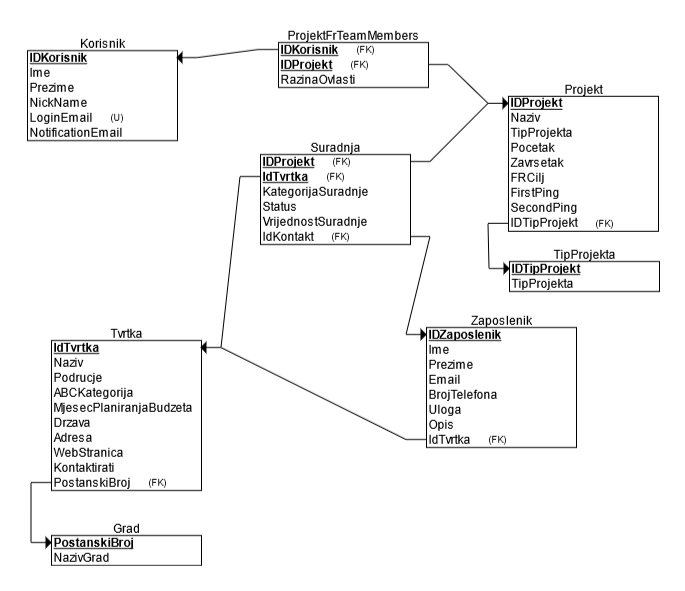
\includegraphics[scale=0.6]{DBDiagram}
					\centering
					\caption{Database Diagram}
					\label{fig:dbdiagram}
				\end{figure}
			\eject
			
			
		\section{Dijagram razreda}
		
			Na sljedećim slikama prikazani su UML dijagrami razreda koji se koriste u aplikaciji. Podijeljeni su u 3 dijela. Prvi dijagram prikazuje klase kojima smo modelirali entitete aplikacije, drugi prikazuje DTO-ove\textit{(Data transfer object)}, a treći prikazuje Controllere. Može se uočiti da postoje veze između klasa iz različitih dijagrama(npr. UserDto sadrži UserSystemAuthority), ali su one izostavljene radi preglednosti.
			
			\begin{figure}[H]
				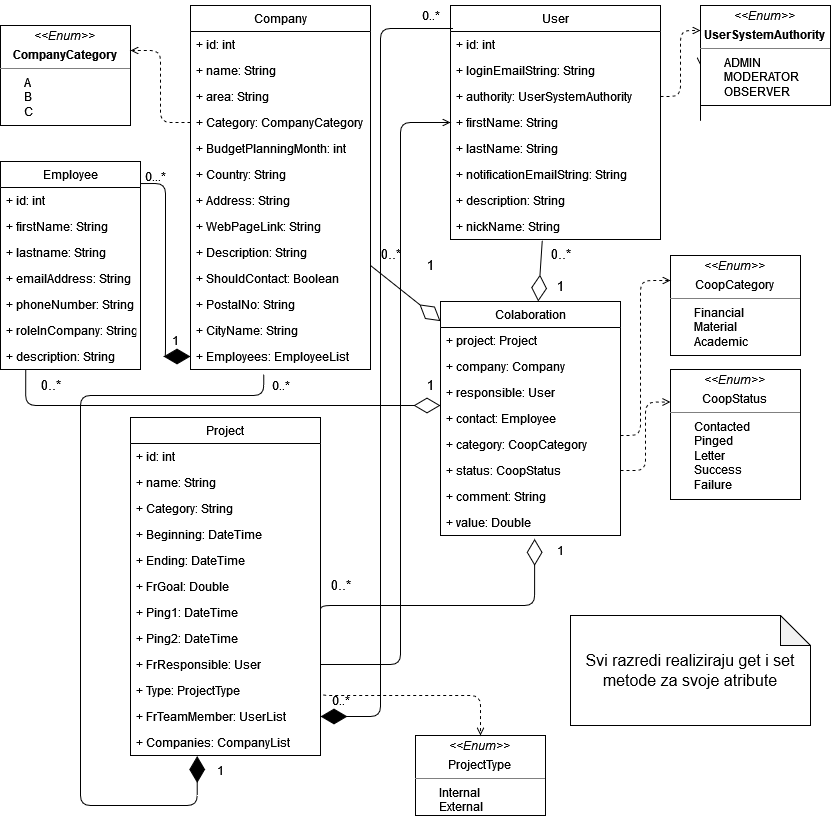
\includegraphics[scale=0.5]{ModelUml} %veličina slike u odnosu na originalnu datoteku i pozicija slike
				\centering
				\caption{Models UML}
				\label{fig:modelUml}
			\end{figure}
			\begin{figure}[H]
				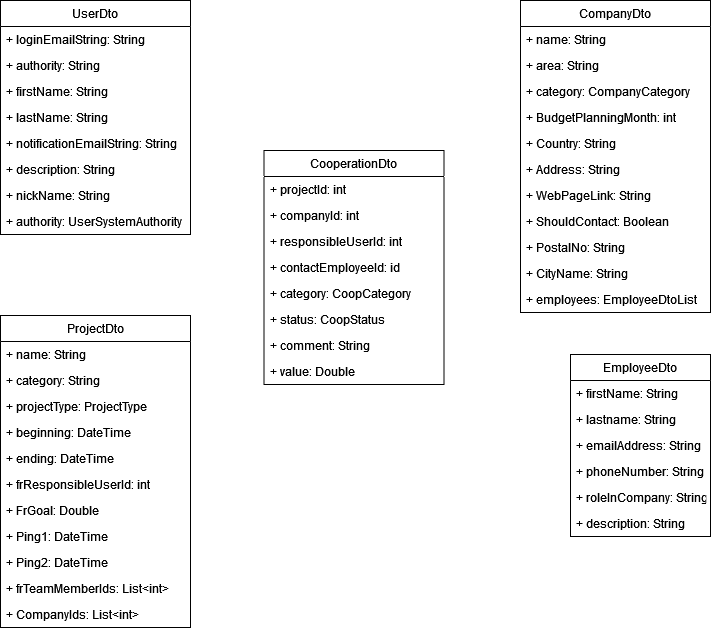
\includegraphics[scale=0.5]{DtoUml} %veličina slike u odnosu na originalnu datoteku i pozicija slike
				\centering
				\caption{DtoUml}
				\label{fig:dtouml}
			\end{figure}
			\begin{figure}[H]
				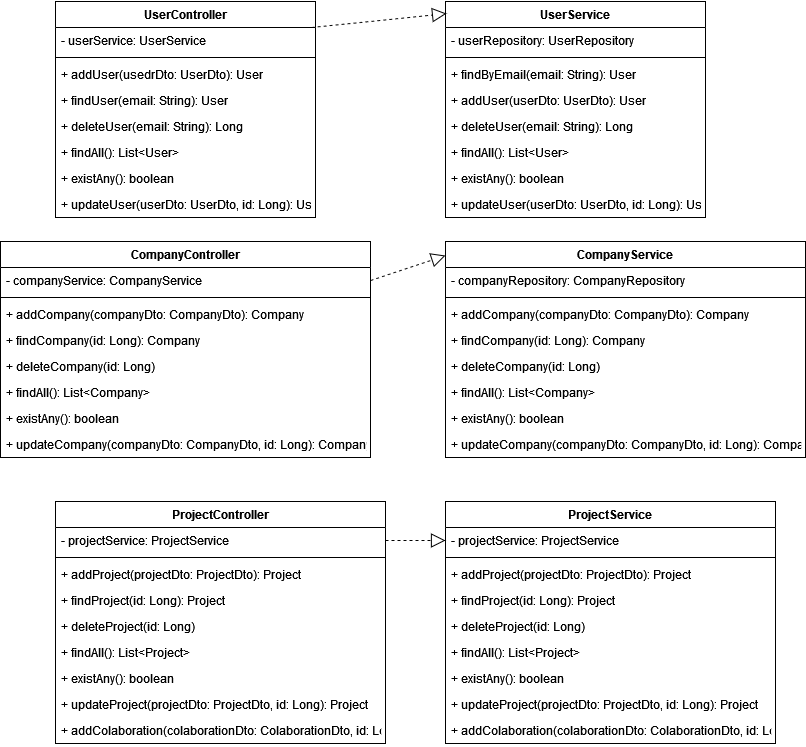
\includegraphics[scale=0.5]{ControllerServiceUml} %veličina slike u odnosu na originalnu datoteku i pozicija slike
				\centering
				\caption{Controllers and services UML}
				\label{fig:controllersServicesUml}
		\end{figure}
		\section{Dijagram stanja}
			
			
			\textbf{\textit{dio 2. revizije}}\\
			
			\textit{Potrebno je priložiti dijagram stanja i opisati ga. Dovoljan je jedan dijagram stanja koji prikazuje \textbf{značajan dio funkcionalnosti} sustava. Na primjer, stanja korisničkog sučelja i tijek korištenja neke ključne funkcionalnosti jesu značajan dio sustava, a registracija i prijava nisu. }
			
			
			\eject 
		
		\section{Dijagram aktivnosti}
			
			\textbf{\textit{dio 2. revizije}}\\
			
			 \textit{Potrebno je priložiti dijagram aktivnosti s pripadajućim opisom. Dijagram aktivnosti treba prikazivati značajan dio sustava.}
			
			\eject
		\section{Dijagram komponenti}
		
			\textbf{\textit{dio 2. revizije}}\\
		
			 \textit{Potrebno je priložiti dijagram komponenti s pripadajućim opisom. Dijagram komponenti treba prikazivati strukturu cijele aplikacije.}